\noindent

%%%%%%%%%% CÂU 1 %%%%%%%%%%
{\normalcolor{\textbf{CÂU I. (4.0 điểm)}}}
\setcounter{equation}{0}


Cho một sợi dây thép cứng, nhẵn được uốn thành đa giác lồi $N$ cạnh có chiều dài các cạnh là $l_1, l_2,..., l_N$ và mặt bàn nhẵn nằm ngang có hình dạng giống hệt đa giác ở trên.
\begin{enumerate}[label=(\alph*)]
\item Ta uốn sợi dây thành đa giác đều ($l_1=l_2=...=l_N=l$). Giả sử rằng ta có $N$ ròng rọc rất nhỏ và rất nhẹ luồn vào từng cạnh của đa giác, sau đó buộc $N$ sợi dây nhẹ, không dãn sao cho một đầu được nối vào quả nặng $M$, đầu còn lại được nối vào những khối lượng bằng nhau có khối lượng $m$. Đặt khối lượng $M$ lên bàn và vắt mỗi sợi dây lên các ròng rọc có chỉ số các cạnh tương ứng (như hình vẽ bên dưới). Xét trong vùng mà mỗi cạnh của đa giác chỉ chứa một ròng rọc, hãy xác định các vị trí cân bằng trong khu vực này. Vẽ hình chỉ ra vị trí cân bằng cho trường hợp $N=5$ và $N=6$.

\begin{figure}[!h]
    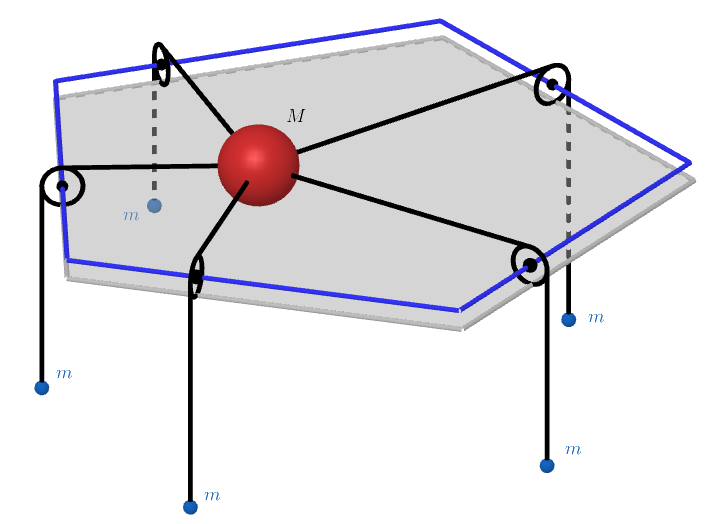
\includegraphics[width=0.5\linewidth]{Problem_1/Figs_P1/Figs_P1.png}
    \centering
    \label{fig:P1_01}
    \caption{}
\end{figure}
\item Xét trường hợp $N = 3$ (nói cách khác là cuốn sợi dây thành hình tam giác có cạnh $l_1, l_2, l_3$), sau đó luồn 3 hạt cườm rất nhẹ vào mỗi cạnh, mỗi hạt cườm lại có một lò xo có độ dài tự nhiên rất nhỏ (coi bằng 0) có độ cứng $k_1, k_2, k_3$ và một đầu của mỗi lò xo được gắn vào khối lượng $M$ (như hình ở dưới). Đặt vật $M$ trên bàn. Xác định vị trí cân bằng trong các trường hợp:
    \begin{enumerate}[label=(\roman*)]
    \item Độ dài các cạnh của tam giác và các độ cứng của lò xo thỏa mãn: $l_1:l_2:l_3=k_1:k_2:k_3$.
    \item Các độ cứng của lò xo bằng nhau và bằng $k$.
    \end{enumerate}
\begin{figure}[H]
    \centering
    % Gradient Info
  
\tikzset {_2c9ddldf2/.code = {\pgfsetadditionalshadetransform{ \pgftransformshift{\pgfpoint{89.1 bp } { -128.7 bp }  }  \pgftransformscale{1.32 }  }}}
\pgfdeclareradialshading{_8o830cp2v}{\pgfpoint{-72bp}{104bp}}{rgb(0bp)=(0.89,0.75,0.75);
rgb(0bp)=(0.89,0.75,0.75);
rgb(12.589285714285714bp)=(0.82,0.01,0.11);
rgb(400bp)=(0.82,0.01,0.11)}
\tikzset{every picture/.style={line width=0.75pt}} %set default line width to 0.75pt        

\begin{tikzpicture}[x=0.75pt,y=0.75pt,yscale=-1,xscale=1]
%uncomment if require: \path (0,462); %set diagram left start at 0, and has height of 462

%Shape: Triangle [id:dp3326541587702424] 
\draw  [color={rgb, 255:red, 74; green, 93; blue, 226 }  ,draw opacity=1 ][fill={rgb, 255:red, 128; green, 128; blue, 128 }  ,fill opacity=0.1 ][line width=3]  (179.94,26) -- (429,269.11) -- (50,269.11) -- cycle ;
%Shape: Inductor (Air Core) [id:dp6872930774599556] 
\draw  [line width=1.5]  (206.28,201.94) -- (206.02,213.91) .. controls (209.3,214.15) and (212.07,215.88) .. (213,218.25) .. controls (213.93,220.62) and (212.83,223.16) .. (210.23,224.64) .. controls (208.2,225.79) and (205.6,226.21) .. (203.09,225.82) .. controls (202.11,225.8) and (201.33,225.18) .. (201.35,224.45) .. controls (201.36,223.71) and (202.17,223.14) .. (203.15,223.16) .. controls (205.67,222.87) and (208.25,223.41) .. (210.23,224.64) .. controls (212.33,226.07) and (213.5,228.02) .. (213.45,230.03) .. controls (213.41,232.05) and (212.16,233.94) .. (209.99,235.28) .. controls (207.97,236.42) and (205.37,236.85) .. (202.86,236.45) .. controls (201.88,236.43) and (201.1,235.82) .. (201.12,235.08) .. controls (201.13,234.35) and (201.94,233.77) .. (202.92,233.79) .. controls (205.44,233.51) and (208.02,234.05) .. (209.99,235.28) .. controls (212.1,236.71) and (213.26,238.66) .. (213.22,240.67) .. controls (213.18,242.68) and (211.93,244.58) .. (209.76,245.91) .. controls (207.73,247.06) and (205.14,247.49) .. (202.63,247.09) .. controls (201.65,247.07) and (200.87,246.45) .. (200.88,245.72) .. controls (200.9,244.99) and (201.71,244.41) .. (202.69,244.43) .. controls (205.21,244.14) and (207.79,244.68) .. (209.76,245.91) .. controls (212.3,247.51) and (213.28,250.09) .. (212.25,252.42) .. controls (211.22,254.75) and (208.38,256.35) .. (205.09,256.45) -- (204.83,268.42) ;
%Shape: Inductor (Air Core) [id:dp16634280228018206] 
\draw  [line width=1.5]  (110.6,158.34) -- (126.29,165.64) .. controls (128.31,161.89) and (132.02,159.61) .. (135.64,159.89) .. controls (139.25,160.17) and (142.04,162.96) .. (142.66,166.91) .. controls (143.12,169.99) and (142.34,173.32) .. (140.52,176.06) .. controls (139.99,177.21) and (138.77,177.79) .. (137.81,177.34) .. controls (136.85,176.89) and (136.5,175.59) .. (137.04,174.44) .. controls (137.96,171.28) and (140.01,168.54) .. (142.66,166.91) .. controls (145.63,165.25) and (148.82,165.01) .. (151.46,166.23) .. controls (154.09,167.46) and (155.96,170.05) .. (156.6,173.4) .. controls (157.06,176.48) and (156.29,179.81) .. (154.46,182.55) .. controls (153.93,183.7) and (152.71,184.27) .. (151.75,183.83) .. controls (150.79,183.38) and (150.44,182.08) .. (150.98,180.93) .. controls (151.9,177.77) and (153.95,175.03) .. (156.6,173.4) .. controls (159.58,171.74) and (162.76,171.49) .. (165.4,172.72) .. controls (168.04,173.95) and (169.9,176.54) .. (170.54,179.89) .. controls (171.01,182.96) and (170.23,186.3) .. (168.41,189.04) .. controls (167.87,190.19) and (166.66,190.76) .. (165.69,190.31) .. controls (164.73,189.86) and (164.39,188.57) .. (164.92,187.42) .. controls (165.85,184.26) and (167.89,181.51) .. (170.54,179.89) .. controls (173.97,177.81) and (177.89,178.15) .. (180.44,180.74) .. controls (182.98,183.32) and (183.63,187.63) .. (182.06,191.59) -- (197.75,198.88) ;
%Shape: Inductor (Air Core) [id:dp3092264128133372] 
\draw  [line width=1.5]  (206.35,197.88) -- (221.06,185.93) .. controls (218.69,182.58) and (218.53,178.21) .. (220.65,174.91) .. controls (222.77,171.61) and (226.73,170.06) .. (230.65,171.01) .. controls (233.68,171.76) and (236.31,173.78) .. (237.87,176.55) .. controls (238.64,177.5) and (238.53,178.86) .. (237.63,179.6) .. controls (236.72,180.33) and (235.37,180.16) .. (234.6,179.21) .. controls (232.2,177.12) and (230.76,174.13) .. (230.65,171.01) .. controls (230.67,167.56) and (232.08,164.47) .. (234.56,162.46) .. controls (237.03,160.45) and (240.35,159.7) .. (243.72,160.38) .. controls (246.76,161.13) and (249.39,163.15) .. (250.94,165.93) .. controls (251.71,166.88) and (251.61,168.24) .. (250.7,168.97) .. controls (249.8,169.71) and (248.44,169.53) .. (247.67,168.58) .. controls (245.28,166.49) and (243.84,163.5) .. (243.72,160.38) .. controls (243.75,156.94) and (245.16,153.85) .. (247.64,151.84) .. controls (250.11,149.82) and (253.43,149.07) .. (256.8,149.76) .. controls (259.84,150.51) and (262.47,152.53) .. (264.02,155.3) .. controls (264.79,156.25) and (264.68,157.62) .. (263.78,158.35) .. controls (262.88,159.08) and (261.52,158.91) .. (260.75,157.96) .. controls (258.36,155.87) and (256.92,152.88) .. (256.8,149.76) .. controls (256.68,145.73) and (259.01,142.17) .. (262.67,140.77) .. controls (266.33,139.37) and (270.58,140.42) .. (273.37,143.43) -- (288.08,131.48) ;
%Flowchart: Delay [id:dp8143670880210933] 
\draw  [fill={rgb, 255:red, 0; green, 0; blue, 0 }  ,fill opacity=1 ] (109.35,153.2) -- (112.55,155.15) .. controls (114.31,156.22) and (114.87,158.52) .. (113.8,160.28) .. controls (112.73,162.05) and (110.43,162.61) .. (108.66,161.54) -- (105.47,159.59) -- cycle ;
%Flowchart: Delay [id:dp9198941962672681] 
\draw  [fill={rgb, 255:red, 0; green, 0; blue, 0 }  ,fill opacity=1 ] (200.88,271.94) -- (201.1,268.2) .. controls (201.22,266.14) and (202.99,264.57) .. (205.05,264.69) .. controls (207.11,264.81) and (208.68,266.58) .. (208.56,268.64) -- (208.35,272.37) -- cycle ;
%Flowchart: Delay [id:dp3222573149762976] 
\draw  [fill={rgb, 255:red, 0; green, 0; blue, 0 }  ,fill opacity=1 ] (293.37,131.19) -- (290.87,133.97) .. controls (289.49,135.51) and (287.12,135.64) .. (285.59,134.26) .. controls (284.05,132.88) and (283.92,130.51) .. (285.3,128.98) -- (287.8,126.19) -- cycle ;
%Flowchart: Connector [id:dp4674995309000146] 
\path  [shading=_8o830cp2v,_2c9ddldf2] (196.75,197.88) .. controls (196.75,192.58) and (201.05,188.29) .. (206.35,188.29) .. controls (211.64,188.29) and (215.94,192.58) .. (215.94,197.88) .. controls (215.94,203.18) and (211.64,207.47) .. (206.35,207.47) .. controls (201.05,207.47) and (196.75,203.18) .. (196.75,197.88) -- cycle ; % for fading 
 \draw  [color={rgb, 255:red, 208; green, 2; blue, 27 }  ,draw opacity=1 ][line width=0.75]  (196.75,197.88) .. controls (196.75,192.58) and (201.05,188.29) .. (206.35,188.29) .. controls (211.64,188.29) and (215.94,192.58) .. (215.94,197.88) .. controls (215.94,203.18) and (211.64,207.47) .. (206.35,207.47) .. controls (201.05,207.47) and (196.75,203.18) .. (196.75,197.88) -- cycle ; % for border 


% Text Node
\draw (230.7,278.69) node [anchor=north west][inner sep=0.75pt]    {$l_{1}$};
% Text Node
\draw (318.07,126.28) node [anchor=north west][inner sep=0.75pt]    {$l_{2}$};
% Text Node
\draw (86.23,124.46) node [anchor=north west][inner sep=0.75pt]    {$l_{3}$};
% Text Node
\draw (214.79,226.02) node [anchor=north west][inner sep=0.75pt]    {$k_{1}$};
% Text Node
\draw (222.27,133.76) node [anchor=north west][inner sep=0.75pt]    {$k_{2}$};
% Text Node
\draw (142.48,142.07) node [anchor=north west][inner sep=0.75pt]    {$k_{3}$};
% Text Node
\draw (217.94,201.28) node [anchor=north west][inner sep=0.75pt]    {$M$};
\end{tikzpicture}
\centering
\caption{}
\label{fig:P1_02}
\end{figure}
\end{enumerate}

Gợi ý: Có thể sử dụng định lý con nhím cho đa giác $N$ cạnh, tức là: 
\begin{equation}
l_1\vec{\hat{n}_1}+l_2\vec{\hat{n}_2}+...+l_N\vec{\hat{n}_N}=\vec{0}.
\end{equation}
Trong đó $\vec{\hat{n}_i}$ là vector đơn vị pháp tuyến với cạnh thứ $i$, hướng ra ngoài đa giác.

Hoặc có thể sử dụng việc vật đạt trạng thái cân bằng (bền) thì thế năng sẽ đạt giá trị cực tiểu.
\begin{flushright}
    (biên soạn bởi DMQ và Carina)
\end{flushright}
\newpage

%%%%%%%%%% CÂU 2 %%%%%%%%%%
{\normalcolor{\textbf{CÂU II. (4.0 điểm)}}\vspace{1.5mm}}
\setcounter{equation}{0}


Nguyên lý Scheimpflug được đặt theo tên của kỹ sư người Áo Theodor Scheimpflug, mô tả cách một mặt phẳng tiêu cự có thể nghiêng để mở rộng vùng ảnh rõ nét trong nhiếp ảnh và quang học. 

Cụ thể, nguyên lý Scheimpflug phát biểu rằng khi mặt phẳng vật, mặt phẳng thấu kính và mặt phẳng ảnh (cảm biến hoặc phim) không song song mà giao nhau tại một đường thẳng chung, thì toàn bộ mặt phẳng vật nghiêng này vẫn có thể được lấy nét rõ ràng. 
\begin{enumerate}[label=(\alph*)]
\item Chứng minh nguyên lý Scheimpflug
\item Chứng minh rằng mặt phẳng tiêu cự quay quanh một trục đi qua điểm G khi ta nghiêng thấu kính \\
\begin{figure}[H]
    \centering
    \tikzset{every picture/.style={line width=0.75pt}} %set default line width to 0.75pt        

\begin{tikzpicture}[x=0.75pt,y=0.75pt,yscale=-1,xscale=1]
%uncomment if require: \path (0,424); %set diagram left start at 0, and has height of 424

%Straight Lines [id:da17793481393532118] 
\draw    (100,106) -- (411,330) ;
%Straight Lines [id:da4232639599589497] 
\draw    (411,88) -- (411,330) ;
%Straight Lines [id:da11938100176501354] 
\draw    (331,52) -- (411,330) ;
%Straight Lines [id:da838504233570497] 
\draw [color={rgb, 255:red, 215; green, 208; blue, 208 }  ,draw opacity=1 ]   (108,111) -- (411,209) ;
%Straight Lines [id:da49314275647124217] 
\draw [color={rgb, 255:red, 215; green, 208; blue, 208 }  ,draw opacity=1 ]   (255.5,218) -- (411,189) ;
%Straight Lines [id:da48246879037954804] 
\draw [color={rgb, 255:red, 14; green, 39; blue, 252 }  ,draw opacity=1 ]   (372,49) -- (373,360) ;
%Curve Lines [id:da20103497237081303] 
\draw [color={rgb, 255:red, 14; green, 39; blue, 252 }  ,draw opacity=1 ]   (195,174) .. controls (223.86,123.25) and (302.21,77.46) .. (370.96,92.76) ;
\draw [shift={(372,93)}, rotate = 193.06] [color={rgb, 255:red, 14; green, 39; blue, 252 }  ,draw opacity=1 ][line width=0.75]    (10.93,-3.29) .. controls (6.95,-1.4) and (3.31,-0.3) .. (0,0) .. controls (3.31,0.3) and (6.95,1.4) .. (10.93,3.29)   ;
%Curve Lines [id:da766499281537382] 
\draw [color={rgb, 255:red, 14; green, 39; blue, 252 }  ,draw opacity=1 ]   (320,77) .. controls (327.6,67.5) and (323.47,70.64) .. (333.32,64.97) ;
\draw [shift={(335,64)}, rotate = 149.74] [color={rgb, 255:red, 14; green, 39; blue, 252 }  ,draw opacity=1 ][line width=0.75]    (10.93,-3.29) .. controls (6.95,-1.4) and (3.31,-0.3) .. (0,0) .. controls (3.31,0.3) and (6.95,1.4) .. (10.93,3.29)   ;
%Curve Lines [id:da17003487311025278] 
\draw [color={rgb, 255:red, 14; green, 39; blue, 252 }  ,draw opacity=1 ]   (391,74) .. controls (386.28,65.49) and (384.23,65.03) .. (373.89,62.47) ;
\draw [shift={(372,62)}, rotate = 14.04] [color={rgb, 255:red, 14; green, 39; blue, 252 }  ,draw opacity=1 ][line width=0.75]    (10.93,-3.29) .. controls (6.95,-1.4) and (3.31,-0.3) .. (0,0) .. controls (3.31,0.3) and (6.95,1.4) .. (10.93,3.29)   ;
%Straight Lines [id:da9027721988306059] 
\draw [color={rgb, 255:red, 14; green, 39; blue, 252 }  ,draw opacity=1 ][fill={rgb, 255:red, 14; green, 39; blue, 252 }  ,fill opacity=1 ]   (293,56) -- (373,302) ;
%Straight Lines [id:da5757635442365009] 
\draw [color={rgb, 255:red, 204; green, 48; blue, 232 }  ,draw opacity=0.79 ]   (221,193) -- (411,197) ;
%Straight Lines [id:da515546325781679] 
\draw [color={rgb, 255:red, 14; green, 39; blue, 252 }  ,draw opacity=1 ]   (373,302) -- (401,294) ;
%Straight Lines [id:da07987517143448997] 
\draw [color={rgb, 255:red, 14; green, 39; blue, 252 }  ,draw opacity=1 ]   (411,197) -- (440,197) ;
%Straight Lines [id:da32954315898274145] 
\draw [color={rgb, 255:red, 14; green, 39; blue, 252 }  ,draw opacity=1 ]   (373,302) -- (440,302) ;
%Straight Lines [id:da7673507644962323] 
\draw [color={rgb, 255:red, 14; green, 39; blue, 252 }  ,draw opacity=1 ]   (440,240) -- (440,199) ;
\draw [shift={(440,197)}, rotate = 90] [color={rgb, 255:red, 14; green, 39; blue, 252 }  ,draw opacity=1 ][line width=0.75]    (10.93,-3.29) .. controls (6.95,-1.4) and (3.31,-0.3) .. (0,0) .. controls (3.31,0.3) and (6.95,1.4) .. (10.93,3.29)   ;
%Straight Lines [id:da3847843275842151] 
\draw [color={rgb, 255:red, 14; green, 39; blue, 252 }  ,draw opacity=1 ]   (440,261) -- (440,300) ;
\draw [shift={(440,302)}, rotate = 270] [color={rgb, 255:red, 14; green, 39; blue, 252 }  ,draw opacity=1 ][line width=0.75]    (10.93,-3.29) .. controls (6.95,-1.4) and (3.31,-0.3) .. (0,0) .. controls (3.31,0.3) and (6.95,1.4) .. (10.93,3.29)   ;
%Straight Lines [id:da20281608213079083] 
\draw [color={rgb, 255:red, 14; green, 39; blue, 252 }  ,draw opacity=1 ]   (221,193) -- (221,361) ;
%Straight Lines [id:da1408913001205767] 
\draw [color={rgb, 255:red, 14; green, 39; blue, 252 }  ,draw opacity=1 ]   (411,330) -- (411,361) ;
%Straight Lines [id:da8412446681679657] 
\draw [color={rgb, 255:red, 14; green, 39; blue, 252 }  ,draw opacity=1 ]   (290,360) -- (223,360.97) ;
\draw [shift={(221,361)}, rotate = 359.17] [color={rgb, 255:red, 14; green, 39; blue, 252 }  ,draw opacity=1 ][line width=0.75]    (10.93,-3.29) .. controls (6.95,-1.4) and (3.31,-0.3) .. (0,0) .. controls (3.31,0.3) and (6.95,1.4) .. (10.93,3.29)   ;
%Straight Lines [id:da9709846088927524] 
\draw [color={rgb, 255:red, 14; green, 39; blue, 252 }  ,draw opacity=1 ]   (317,360) -- (371,360) ;
\draw [shift={(373,360)}, rotate = 180] [color={rgb, 255:red, 14; green, 39; blue, 252 }  ,draw opacity=1 ][line width=0.75]    (10.93,-3.29) .. controls (6.95,-1.4) and (3.31,-0.3) .. (0,0) .. controls (3.31,0.3) and (6.95,1.4) .. (10.93,3.29)   ;
%Straight Lines [id:da3803562259739416] 
\draw [color={rgb, 255:red, 14; green, 39; blue, 252 }  ,draw opacity=1 ]   (398,360) -- (409.01,360.85) ;
\draw [shift={(411,361)}, rotate = 184.4] [color={rgb, 255:red, 14; green, 39; blue, 252 }  ,draw opacity=1 ][line width=0.75]    (10.93,-3.29) .. controls (6.95,-1.4) and (3.31,-0.3) .. (0,0) .. controls (3.31,0.3) and (6.95,1.4) .. (10.93,3.29)   ;
%Straight Lines [id:da20928323034235796] 
\draw [color={rgb, 255:red, 14; green, 39; blue, 252 }  ,draw opacity=1 ]   (388,360) -- (375,360) ;
\draw [shift={(373,360)}, rotate = 360] [color={rgb, 255:red, 14; green, 39; blue, 252 }  ,draw opacity=1 ][line width=0.75]    (10.93,-3.29) .. controls (6.95,-1.4) and (3.31,-0.3) .. (0,0) .. controls (3.31,0.3) and (6.95,1.4) .. (10.93,3.29)   ;

% Text Node
\draw (346,55.4) node [anchor=north west][inner sep=0.75pt]    {$\theta $};
% Text Node
\draw (258,82.4) node [anchor=north west][inner sep=0.75pt]    {$\psi $};
% Text Node
\draw (356,301.4) node [anchor=north west][inner sep=0.75pt]    {$\text{G}$};
% Text Node
\draw (77,86.4) node [anchor=north west][inner sep=0.75pt]    {$\text{PoF}$};
% Text Node
\draw (269,39.4) node [anchor=north west][inner sep=0.75pt]    {$\text{FP}$};
% Text Node
\draw (315,33.4) node [anchor=north west][inner sep=0.75pt]    {$\text{LP}$};
% Text Node
\draw (406,66.4) node [anchor=north west][inner sep=0.75pt]    {$\text{IP}$};
% Text Node
\draw (413,333.4) node [anchor=north west][inner sep=0.75pt]    {$\text{S}$};
% Text Node
\draw (377,280.4) node [anchor=north west][inner sep=0.75pt]    {$\text{f}$};
% Text Node
\draw (431,240.4) node [anchor=north west][inner sep=0.75pt]    {$\text{J}$};
% Text Node
\draw (297,348.4) node [anchor=north west][inner sep=0.75pt]    {$\text{u'}$};
% Text Node
\draw (386,349.4) node [anchor=north west][inner sep=0.75pt]    {$\text{v'}$};
\end{tikzpicture}
\centering
\caption{}
    \label{fig:P2_01}
\end{figure}
\begin{enumerate}[label={}]
    \item IP=mặt phẳng ảnh
    \item LP=mặt phẳng thấu kính
    \item FP=mặt phẳng tiêu điểm trước (mặt phẳng song song LP và đi qua F)
    \item PoF=mặt phẳng tiêu cự
\end{enumerate}
\end{enumerate}
Một nghiên cứu sử dụng nguyên lý Scheimpflug và hệ thấu kính nghiêng để mô hình hóa hình dạng 3D của đồ vật. Bằng cách đặt vật thể trên một bệ dịch chuyển và cho chuyển động thẳng với tốc độ đồng đều rồi chụp ở mọi khoảng cách đã định, ta sẽ ghi lại được đường nét của vật. Bố trí thí nghiệm của nghiên cứu được cho ở hình vẽ bên dưới: 
\begin{figure}[H]
    \centering
   \begin{tikzpicture}[x=0.75pt,y=0.75pt,yscale=-1,xscale=1]
% Uncomment if required: \path (0,424); % set diagram left start at 0, and has height of 424

% Shape: Parallelogram [id:dp00958650764397817] 
\draw [fill={rgb, 255:red, 19; green, 161; blue, 184}, fill opacity=1] 
  (181.39,232.64) -- (124.36,214.59) -- (123.88,249.83) -- (180.91,267.88) -- cycle ;

% Shape: Parallelogram [id:dp022474278506247614] 
\draw [fill={rgb, 255:red, 13; green, 245; blue, 189}, fill opacity=1] 
  (276.57,195.97) -- (175.86,164.08) -- (176.78,228.21) -- (277.49,260.1) -- cycle ;

% Straight Lines [id:da8907782196447741]
\draw (260.02,254.57) -- (358.33,285) ;

% Shape: Ellipse [id:dp05488901106901134]
\draw [fill={rgb, 255:red, 255; green, 0; blue, 128}, fill opacity=1] 
  (358.33,285)
  .. controls (358.33,278.92) and (362.36,274) .. (367.33,274)
  .. controls (372.3,274) and (376.33,278.92) .. (376.33,285)
  .. controls (376.33,291.08) and (372.3,296) .. (367.33,296)
  .. controls (362.36,296) and (358.33,291.08) .. (358.33,285) -- cycle ;

% Straight Lines [id:da7460212634378354]
\draw [color={rgb, 255:red, 174; green, 170; blue, 170}, draw opacity=1]
  (283.47,186.65) -- (367.33,274) ;

% Shape: Triangle [id:dp18484560531905792]
\draw [fill={rgb, 255:red, 225; green, 18; blue, 18}, fill opacity=0.48]
  (419.17,92.13) -- (376.33,285) -- (420.11,210.91) -- cycle ;

% Shape: Parallelogram [id:dp2907384191063157]
\draw [fill={rgb, 255:red, 23; green, 23; blue, 23}, fill opacity=0.14]
  (429.37,91.89) -- (289.7,47.67) -- (292.67,177.78) -- (432.33,222) -- cycle ;

% Shape: Ellipse [id:dp3004682236426569]
\draw [fill={rgb, 255:red, 58; green, 216; blue, 237}, fill opacity=0.75]
  (313.45,207.21)
  .. controls (330.49,225.08) and (344.71,244.84) .. (345.19,251.35)
  .. controls (345.68,257.86) and (332.26,248.65) .. (315.22,230.79)
  .. controls (298.17,212.92) and (283.96,193.16) .. (283.47,186.65)
  .. controls (282.99,180.14) and (296.41,189.35) .. (313.45,207.21) -- cycle ;

% Straight Lines with Arrowheads
\draw (70,260) -- (92.54,248.88);
\draw [shift={(94.33,248)}, rotate=153.75, color=black, line width=0.75]
  (10.93,-3.29) .. controls (6.95,-1.4) and (3.31,-0.3) .. (0,0) 
  .. controls (3.31,0.3) and (6.95,1.4) .. (10.93,3.29);

\draw (70,260) -- (103.37,266.61);
\draw [shift={(105.33,267)}, rotate=191.21, color=black, line width=0.75]
  (10.93,-3.29) .. controls (6.95,-1.4) and (3.31,-0.3) .. (0,0) 
  .. controls (3.31,0.3) and (6.95,1.4) .. (10.93,3.29);

\draw (70,260) -- (70.31,286);
\draw [shift={(70.33,288)}, rotate=269.32, color=black, line width=0.75]
  (10.93,-3.29) .. controls (6.95,-1.4) and (3.31,-0.3) .. (0,0) 
  .. controls (3.31,0.3) and (6.95,1.4) .. (10.93,3.29);

\draw (70,260) -- (158.33,245);
\draw (180.33,243) -- (248.33,230);
\draw (70,260) -- (141.33,241);
\draw (177.44,231.29) -- (214.76,222.04);

% Shape: Circle
\draw [fill={rgb, 255:red, 18; green, 16; blue, 16}, fill opacity=1]
  (139.83,241)
  .. controls (139.83,240.17) and (140.5,239.5) .. (141.33,239.5)
  .. controls (142.16,239.5) and (142.83,240.17) .. (142.83,241)
  .. controls (142.83,241.83) and (142.16,242.5) .. (141.33,242.5)
  .. controls (140.5,242.5) and (139.83,241.83) .. (139.83,241) -- cycle ;

\draw [fill={rgb, 255:red, 18; green, 16; blue, 16}, fill opacity=1]
  (156.83,245)
  .. controls (156.83,244.17) and (157.5,243.5) .. (158.33,243.5)
  .. controls (159.16,243.5) and (159.83,244.17) .. (159.83,245)
  .. controls (159.83,245.83) and (159.16,246.5) .. (158.33,246.5)
  .. controls (157.5,246.5) and (156.83,245.83) .. (156.83,245) -- cycle ;

\draw [fill={rgb, 255:red, 18; green, 16; blue, 16}, fill opacity=1]
  (213.26,222.04)
  .. controls (213.26,221.21) and (213.94,220.54) .. (214.76,220.54)
  .. controls (215.59,220.54) and (216.26,221.21) .. (216.26,222.04)
  .. controls (216.26,222.87) and (215.59,223.54) .. (214.76,223.54)
  .. controls (213.94,223.54) and (213.26,222.87) .. (213.26,222.04) -- cycle ;

\draw [fill={rgb, 255:red, 18; green, 16; blue, 16}, fill opacity=1]
  (245.33,230)
  .. controls (245.33,229.17) and (246,228.5) .. (246.83,228.5)
  .. controls (247.66,228.5) and (248.33,229.17) .. (248.33,230)
  .. controls (248.33,230.83) and (247.66,231.5) .. (246.83,231.5) -- cycle ;

\draw (420.33,198) -- (248.33,230);

\draw [fill={rgb, 255:red, 18; green, 16; blue, 16}, fill opacity=1]
  (312.83,217.5)
  .. controls (312.83,216.67) and (313.5,216) .. (314.33,216)
  .. controls (315.16,216) and (315.83,216.67) .. (315.83,217.5)
  .. controls (315.83,218.33) and (315.16,219) .. (314.33,219)
  .. controls (313.5,219) and (312.83,218.33) .. (312.83,217.5) -- cycle ;

\draw (315.83,217.5) -- (420.33,151);
\draw (420.33,198) -- (341.05,244.98);
\draw [shift={(339.33,246)}, rotate=329.35, color=black, line width=0.75]
  (10.93,-3.29) .. controls (6.95,-1.4) and (3.31,-0.3) .. (0,0) 
  .. controls (3.31,0.3) and (6.95,1.4) .. (10.93,3.29);

\draw (246.83,230) -- (299.52,205.83);
\draw [shift={(301.33,205)}, rotate=155.36, color=black, line width=0.75]
  (10.93,-3.29) .. controls (6.95,-1.4) and (3.31,-0.3) .. (0,0)
  .. controls (3.31,0.3) and (6.95,1.4) .. (10.93,3.29);

\draw (246.83,230) -- (247.33,245);
\draw (247.33,245) -- (312.48,218.26);
\draw [shift={(314.33,217.5)}, rotate=157.68, color=black, line width=0.75]
  (10.93,-3.29) .. controls (6.95,-1.4) and (3.31,-0.3) .. (0,0)
  .. controls (3.31,0.3) and (6.95,1.4) .. (10.93,3.29);

\draw (420.33,198) -- (420.33,153);
\draw [shift={(420.33,151)}, rotate=90, color=black, line width=0.75]
  (10.93,-3.29) .. controls (6.95,-1.4) and (3.31,-0.3) .. (0,0)
  .. controls (3.31,0.3) and (6.95,1.4) .. (10.93,3.29);

\draw (420.33,151) -- (420.33,196);
\draw [shift={(420.33,198)}, rotate=270, color=black, line width=0.75]
  (10.93,-3.29) .. controls (6.95,-1.4) and (3.31,-0.3) .. (0,0)
  .. controls (3.31,0.3) and (6.95,1.4) .. (10.93,3.29);

\draw [fill={rgb, 255:red, 18; green, 16; blue, 16}, fill opacity=1]
  (245.83,245)
  .. controls (245.83,244.17) and (246.5,243.5) .. (247.33,243.5)
  .. controls (248.16,243.5) and (248.83,244.17) .. (248.83,245)
  .. controls (248.83,245.83) and (248.16,246.5) .. (247.33,246.5)
  .. controls (246.5,246.5) and (245.83,245.83) .. (245.83,245) -- cycle ;

\draw (246.83,228.5) -- (253.33,242);
\draw (251,237) -- (257.33,234);
\draw (257.33,234) -- (260.33,240);

% Text Nodes
\draw (47,246.4) node [anchor=north west, inner sep=0.75pt] {$\text{O}_{c}$};
\draw (82,227.4) node [anchor=north west, inner sep=0.75pt] {$\text{Z}_{c}$};
\draw (105.33,264.4) node [anchor=north west, inner sep=0.75pt] {$\text{X}_{c}$};
\draw (64,291.4) node [anchor=north west, inner sep=0.75pt] {$\text{Y}_{c}$};
\draw (186,206.4) node [anchor=north west, inner sep=0.75pt] {$\text{f}$};
\draw (236.33,217.4) node [anchor=north west, inner sep=0.75pt, font=\footnotesize] {$\text{P}'$};
\draw (263,200.4) node [anchor=north west, inner sep=0.75pt] {$\text{l}'$};
\draw (438,165.4) node [anchor=north west, inner sep=0.75pt] {$\text{h}$};
\draw (282.83,234.65) node [anchor=north west, inner sep=0.75pt] {$\text{l}'_{0}$};
\draw (310.83,193.9) node [anchor=north west, inner sep=0.75pt, font=\scriptsize] {$\text{O}_{m}$};
\draw (237,231.4) node [anchor=north west, inner sep=0.75pt, font=\scriptsize] {$\text{x}$};
\draw (230.33,249.9) node [anchor=north west, inner sep=0.75pt, font=\footnotesize] {$\text{Q}'$};
\draw (256.44,242.28) node [anchor=north west, inner sep=0.75pt, font=\scriptsize] {$\text{M}$};
\draw (435,198.4) node [anchor=north west, inner sep=0.75pt] {$\text{P}$};
\draw (434,140.4) node [anchor=north west, inner sep=0.75pt] {$\text{Q}$};
\draw (372,227.4) node [anchor=north west, inner sep=0.75pt] {$\text{l}$};
\draw (349,166.4) node [anchor=north west, inner sep=0.75pt] {$\text{l}_{0}$};
\draw (160.33,246.9) node [anchor=north west, inner sep=0.75pt, font=\footnotesize] {$\text{P}''$};

\end{tikzpicture}

    \caption{}
    \label{fig:P2_02}
\end{figure}
\begin{enumerate}[label=(\alph*)]
\addtocounter{enumi}{2}
\item Tìm h theo x, $\alpha$, l, $\beta$, và l’. Cho biết l và l' là khoảng cách từ P và P' đến trục thấu kính, $l_0$ và $l_0'$ là khoảng cách từ Q và Q' đến trục thấu kính, $\alpha$ là góc giữa mặt phẳng ảnh chứa P' và Q' và mặt phẳng thấu kính, $\beta$ là góc giữa mặt phẳng thấu kính và mặt phẳng laser màu đỏ. \\
Biết $\sin x \cos y+\cos x \sin y=\sin{(y+x)}$
\item Biểu diễn tọa độ của điểm P trong hệ tọa độ $O_cX_cY_cZ_c$ gắn với camera. Biết tọa độ điểm P" là ($x^"_C, y^"_C, z^"_C$)\\ 
Cho biết phương trình tham số đường thẳng đi qua hai điểm A và B bất kì có dạng: 
\setcounter{equation}{0}
\begin{equation}
    \begin{cases}
    x = (x_A - x_B)t + x_A \\
    y = (y_A - y_B)t + y_A \\
    z = (z_A - z_B)t + z_A
\end{cases}
\end{equation}
Và phương trình mô tả mặt phẳng màn (phần màu xám) trong hệ tọa độ $O_cX_cY_cZ_c$ có dạng: 
\begin{equation}
    A_cx+B_cy+C_cz+D_1=0
\end{equation}
Các điểm có tọa độ thỏa mãn phương trình trên sẽ nằm trên màn.
\end{enumerate}
Bằng cách xác định tọa độ điểm $P$ và phương trình biểu diễn mặt phẳng ánh sáng, ta có thể vạch ra hình dạng 3D của vật thể.

\begin{flushright}
    (biên soạn bởi Meng)
\end{flushright}
\newpage

%%%%%%%%%% CÂU 3 %%%%%%%%%%
{\normalcolor{\textbf{CÂU III. (4.0 điểm)}}}
\setcounter{equation}{0}

Graphite là một dạng carbon có cấu trúc lớp, trong đó các lớp carbon liên kết với nhau bằng liên kết cộng hóa trị, tạo ra tính dẫn điện tốt. Do đó, graphite được sử dụng trong nhiều ứng dụng điện tử và công nghiệp. Trong bài tập này, mục tiêu sẽ là đo điện trở của graphite để nghiên cứu sự thay đổi của điện trở theo các yếu tố như kích thước, nhiệt độ vật liệu.\\
Ta sẽ khảo sát sự phụ thuộc của điện trở của graphite $R_g$ vào nhiệt độ của nó. Sự phụ thuộc này có thể được xấp xỉ là tuyến tính theo biểu thức sau:
\begin{equation}
    R_g=R_0(1+\alpha \Delta T).
\end{equation}
Với $\Delta T$ là chênh lệch nhiệt độ giữa phòng và graphite, $R_0$ là điện trở graphite ở nhiệt độ phòng, $\alpha$ là một hằng số.
Ngoài ra, giả sử rằng công suất truyền nhiệt ra môi trường tỉ lệ thuận với chênh lệch nhiệt độ giữa môi trường và thanh được cho bằng biểu thức:
$P=\beta \Delta T $ ($\beta$ là một hằng số). \\
Mạch được sử dụng cho thí nghiệm cho như hình bên dưới: 
\begin{figure}[h]
\ctikzset{resistor = european}
\centering
\begin{circuitikz}
\draw (0,0) to[battery] (0,3);

\draw (0,3) -- (1.5,3);
\draw (1.5,3) -- (2,3); 
\draw (2,3) to[R=$R_g$] (4,3)
           to[R=$R_0$] (6,3);

\draw (6,3) -- (6.5,3);

\draw (4,3) to[rmeter, t=V] (4,4.8);
\draw (4,4.8) node[ocirc]{};

\draw (6.5,3) -- (8,3) to[vR=$R$] (8,0) -- (0,0);

\draw (1.5,3) |- (3.8,5);
\draw (3.8,5) node[ocirc]{};
\draw (3.6,5.2) node{1}; 

\draw (6.5,3) |- (4.2,5);
\draw (4.2,5) node[ocirc]{};
\draw (4.4,5.2) node{2}; 
\end{circuitikz}
\caption{Mạch điện đo điện trở $R_g$}
\end{figure}
Dụng cụ và thiết bị được sử dụng: thanh graphite, đồng hồ đo điện, nguồn điện (pin 4.5 V), điện trở cố định 1.0 $\Omega$ và 10 $\Omega$ (kí hiệu là $R_0)$, biến trở $R$, dây nối, đồng hồ bấm giờ, bình chứa tuyết.
\begin{enumerate}[label=(\alph*)]
\item Từ hình vẽ bố trí thí nghiệm và dụng cụ thí nghiệm, giải thích cách đo.
\newpage 
\item Cho bảng số liệu như sau: 
\begin{figure}[H]
{\large
\begin{tabular}{|c|c|c|c|}
\hline
\textbf{U (V)} & \textbf{I (A)} & \textbf{P (W)} & \textbf{R ($\Omega$)} \\
\hline
0.150 & 0.040 & 0.0060 & 3.750 \\
0.188 & 0.050 & 0.0094 & 3.760 \\
0.202 & 0.054 & 0.0109 & 3.741 \\
0.261 & 0.070 & 0.0183 & 3.729 \\
0.304 & 0.081 & 0.0246 & 3.753 \\
0.411 & 0.109 & 0.0448 & 3.771 \\
0.470 & 0.124 & 0.0583 & 3.790 \\
0.742 & 0.199 & 0.1477 & 3.729 \\
0.907 & 0.243 & 0.2204 & 3.733 \\
1.155 & 0.312 & 0.3604 & 3.702 \\
1.486 & 0.406 & 0.6033 & 3.660 \\
1.570 & 0.430 & 0.6751 & 3.651 \\
2.280 & 0.640 & 1.4592 & 3.563 \\
\hline
\end{tabular}
}
    \centering
    \caption{}
\end{figure}
Vẽ đồ thị đặc tuyến U-I của graphite.
\item Từ lý thuyết, rút ra phương trình mô tả xấp xỉ đặc tuyến U-I ở đồ thị trên, biết rằng với $\alpha$ nhỏ ta có thể xấp xỉ nhỏ như sau: \begin{equation}
    \dfrac{1}{1+k\alpha} \approx (1-k\alpha).
\end{equation}
Với nghiệm của phương trình bậc 2 thu được trong quá trình tính toán, hãy lấy nghiệm nhỏ hơn.
\item Tính điện trở suất của graphite, biết rằng đường kính của sợi graphite sử dụng là $d=1 mm$ và chiều dài là $l= 5cm$.
\item Từ lý thuyết, chứng minh rằng điện trở graphite phụ thuộc vào công suất tỏa nhiệt theo biểu thức:

\begin{equation}
    R_g=R_0(1+\gamma P).
\end{equation}
\newpage
\item Từ số liệu đã cho, tìm $\gamma$.
\item Nếu đặt sợi dây graphite trên vào tuyết, ta thu được số liệu như sau:
\begin{figure}[H]
\large{
\begin{tabular}{|c|c|}
\hline
\textbf{U (V)} & \textbf{I (A)} \\
\hline
0.144 & 0.037 \\
0.177 & 0.045 \\
0.248 & 0.064 \\
0.292 & 0.076 \\
0.354 & 0.091 \\
0.504 & 0.130 \\
0.721 & 0.188 \\
0.895 & 0.232 \\
1.205 & 0.312 \\
1.554 & 0.409 \\
\hline
\end{tabular}
}
    \centering
    \caption{}
\end{figure}
Từ số liệu đã cho, tính $\alpha$.
\end{enumerate}
\begin{flushright}
   (biên soạn bởi Meng)
\end{flushright}
\newpage

%%%%%%%%%% CÂU 4 %%%%%%%%%%
{\normalcolor{\textbf{CÂU IV. (4.0 điểm)}}}
\setcounter{equation}{0}


Một mặt bàn hình vuông có khối lượng m (trọng lượng phân bố đều) và cạnh dài a được treo bằng 4 sợi dây xích đồng nhất và có chiều dài L. Đặt hệ tọa độ có gốc đặt tại trung tâm của bàn, các sợi dây được gắn cố định vào mặt bàn tại 4 góc và các điểm có tọa độ $\left(\pm \frac{a}{2},\pm\frac{a}{2}\right)$. 
\begin{figure}[H]
    \centering
    \tikzset{every picture/.style={line width=0.75pt}} %set default line width to 0.75pt        

\begin{tikzpicture}[x=0.75pt,y=0.75pt,yscale=-1,xscale=1]
%uncomment if require: \path (0,429); %set diagram left start at 0, and has height of 429

%Shape: Rectangle [id:dp43479829147458826] 
\draw   (150,200) -- (350,200) -- (350,220) -- (150,220) -- cycle ;
%Shape: Rectangle [id:dp26418096458424434] 
\draw   (350,200) -- (442.03,122.78) -- (442.03,143.14) -- (350,220) -- cycle ;
%Straight Lines [id:da6303516163988201] 
\draw    (240.42,122.25) -- (442.46,122.25) ;
%Straight Lines [id:da2435007903542885] 
\draw    (149.96,200) -- (240.78,122.42) ;
%Straight Lines [id:da12397037243108167] 
\draw    (112.03,23.59) -- (461.43,23.59) ;
%Shape: Axis 2D [id:dp11255839884999319] 
%\draw [dashed] (121.01,156.7) -- (506.99,156.7)(409.6,45.33) -- (177.57,277.36) (504.99,151.7) -- (506.99,156.7) -- (494.99,161.7) (397.6,52.33) -- (409.6,45.33) -- (407.6,52.33)  ;
%Straight Lines [id:da6910540327628811] 
\draw    (150,200) -- (150,23.64) ;
%Straight Lines [id:da778712219228807] 
\draw    (241,122.34) -- (241,23.55) ;
%Straight Lines [id:da014093703911455924] 
\draw    (442,122.34) -- (442,22.35) ;
%Straight Lines [id:da13741894893199325] 
\draw    (350,200) -- (350,104.51) -- (350,23.64) ;


% Text Node

\filldraw(255.21,171.12) circle(2.5)node [anchor=north east][align=right] {M};

\draw [<->](150,240) -- (250,240)node[below]{a} -- (350,240) ;

\draw [dashed] [->] (165.23,161.12) -- (435.23,161.12);
\draw [dashed] [->] (222.42,232.62) -- (367.93,87.11);
\filldraw(295.21,161.12) circle(2.5) node [anchor=north west][align=left] {O};
\end{tikzpicture}
    \caption{}
    \label{fig:P4_01}
\end{figure}
Giả sử trọng lượng của các dây xích là không đáng kể so với trọng lượng của mặt bàn.
Bên trên mặt bàn, ta đặt một chậu cây có khối lượng M. Đối với bài này, ta coi đế của chậu cây là rất nhỏ so với mặt bàn và coi chậu là một chất điểm M.
\begin{enumerate} [label=(\alph*)]
    \item Khi chậu cây đặt đúng tại tâm bàn và đang cân bằng, giả sử dây không giãn, hãy chứng minh lực căng trong mỗi dây được tính theo công thức:
    \begin{equation}
        T = \dfrac{(m+M)g}{4}
    \end{equation}
\item 
\begin{enumerate}[label=(\roman*)]
\item Đặt chậu cây tại vị trí (x,y), hãy tìm lực căng của từng dây. Coi rằng các dây đều
tuân theo định luật Hooke: $T = k \cdot\Delta{x}$ với $\Delta{x}$ là độ dãn của dây. Cho rằng hệ số đàn hồi k của dây là rất lớn, giới hạn đàn hồi của dây là đủ nhỏ để độ nghiêng của mặt bàn là không đáng kể.
\item Khi không chịu bắt cứ lực căng nào, dây sẽ bị chùng, tìm những vị trí  đặt chậu cây M trên bàn thoả mãn.
\item Dây sẽ bị đứt khi $\Delta{x}>\Delta{l_0}$, tìm quỹ tích các vị trí đặt chậu cây để hệ cân bằng.
\end{enumerate}
\end{enumerate}
\begin{flushright}
    (biên soạn bởi tlonde2675, Khui Đạp Chai và Noozie)
\end{flushright}
\newpage

%%%%%%%%%% CÂU 5 %%%%%%%%%%
{\normalcolor{\textbf{CÂU V. (4.0 điểm)}}}
\setcounter{equation}{0}

\begin{enumerate}[label=(\alph*)]
\item Ta xét một chỏm băng dày. Nếu tại vị trí đó có mật độ dòng nhiệt trung bình tỏa ra ngoài qua bề mặt trái đất là $q = 0.06 \si{W/m^2}$. Tính độ dày $d$ của băng bị tan trong một năm. Biết nhiệt nóng chảy của đá là $L_i =3.4 \times 10^ 5\si{J/kg}$, khối lượng riêng của băng là $\rho_i = 917\si{kg/m^3}$.

\item  Một chỏm băng ở Nam Cực được một nhóm nhà khoa học khám phá trong một chuyến thám hiểm. Khu vực này thông thường là một cao nguyên rộng tuy nhiên lần này họ phát hiện một vùng trũng sâu xuống giống miệng núi lửa. Giả sử rằng, khu vực đó là một hình nón với độ sâu $h = 100\si{m}$, bán kính $r = 500\si{m}$. Băng ở khu vực đó dày $D=2\si{km}$.
Các nhà khoa học sau đó kết luận rằng có một vụ phun trào núi lửa nhỏ ở bên dưới chỏm băng. Khi đó một lượng magma đã thâm nhập vào trong chỏm băng và đông đặc lại khiến cho một lượng băng nào đó tan chảy. Giả sử rằng băng chỉ chuyển động thẳng đứng, magma nóng chảy hoàn toàn và ở $1200 ^{\circ} C$ ở thời điểm đầu. Coi rằng magma sau khi thâm nhập và đông đặc có hình nón ngay bên dưới khu vực bị trũng, thời gian magma dâng lên rất ngắn so với thời gian trao đổi nhiệt và dòng nhiệt chỉ theo phương thẳng đứng.
    \begin{enumerate}[label=(\roman*)]
    \item Trong trạng thái cân bằng thủy tĩnh, chỉ ra rằng nước ở dưới chỏm băng có hình dạng là một hình nón. (Gợi ý: Sử dụng nguyên lí công ảo: Trong trạng thái cân bằng, tổng tất cả công thực hiện đều triệt tiêu mọi di chuyển ảo bất kỳ của cơ hệ hay $\sum \Delta W=0$.)
    \item Giả sử rằng tại mọi thời điểm, phần nước do băng bị chảy là một hình nón. Cùng với các giả thiết bên trên, ta có thể coi rằng sự tan chảy băng được chia làm hai giai đoạn. Đầu tiên, nước ở trên bề mặt magma chưa trong trạng thái cân bằng áp suất vậy nên nó chảy hết ra ngoài (giả sử nước vẫn giữ ở nhiệt độ $0 ^{\circ} C$). Sau đó, trạng thái cân bằng thủy tĩnh được thiết lập. Khi đó nước sẽ chiếm chỗ ở bên trên chỗ bị magma thâm nhập thay vì bị chảy đi (Xem hình vẽ để thấy trạng thái cuối cùng). Sau khi cân bằng nhiệt, hãy xác định: Độ cao $H$ của đỉnh nón nước ở dưới chỏm băng, độ cao $h_1$ của magma đã thâm nhập, tổng khối lượng $m_{tot}$ của nước đã bị tan chảy và khối lượng $m'$ của nước đã chảy ra ngoài. Cho khối lượng riêng của nước: $\rho_w = 1000 \si{kg/m^3}$, khối lượng riêng của đá và magma: $\rho_r = 2900 \si{kg/m^3}$, nhiệt dung riêng của đá và magma: $c_r = 700\si{J/kg.K}$, nhiệt nóng chảy của đá và magma: $L_r = 4.2\times10^5 \si{J/kg}$.
    \end{enumerate}
\begin{figure}[H]
\centering   


% Pattern Info
 
\tikzset{
pattern size/.store in=\mcSize, 
pattern size = 5pt,
pattern thickness/.store in=\mcThickness, 
pattern thickness = 0.3pt,
pattern radius/.store in=\mcRadius, 
pattern radius = 1pt}
\makeatletter
\pgfutil@ifundefined{pgf@pattern@name@_fh87k5v2v}{
\pgfdeclarepatternformonly[\mcThickness,\mcSize]{_fh87k5v2v}
{\pgfqpoint{0pt}{0pt}}
{\pgfpoint{\mcSize+\mcThickness}{\mcSize+\mcThickness}}
{\pgfpoint{\mcSize}{\mcSize}}
{
\pgfsetcolor{\tikz@pattern@color}
\pgfsetlinewidth{\mcThickness}
\pgfpathmoveto{\pgfqpoint{0pt}{0pt}}
\pgfpathlineto{\pgfpoint{\mcSize+\mcThickness}{\mcSize+\mcThickness}}
\pgfusepath{stroke}
}}
\makeatother

% Pattern Info
 
\tikzset{
pattern size/.store in=\mcSize, 
pattern size = 5pt,
pattern thickness/.store in=\mcThickness, 
pattern thickness = 0.3pt,
pattern radius/.store in=\mcRadius, 
pattern radius = 1pt}
\makeatletter
\pgfutil@ifundefined{pgf@pattern@name@_dyu01ch0a lines}{
\pgfdeclarepatternformonly[\mcThickness,\mcSize]{_dyu01ch0a}
{\pgfqpoint{0pt}{0pt}}
{\pgfpoint{\mcSize+\mcThickness}{\mcSize+\mcThickness}}
{\pgfpoint{\mcSize}{\mcSize}}
{\pgfsetcolor{\tikz@pattern@color}
\pgfsetlinewidth{\mcThickness}
\pgfpathmoveto{\pgfpointorigin}
\pgfpathlineto{\pgfpoint{\mcSize}{0}}
\pgfusepath{stroke}}}
\makeatother
\tikzset{every picture/.style={line width=0.75pt}} %set default line width to 0.75pt        

\begin{tikzpicture}[x=0.6pt,y=0.6pt,yscale=-0.7,xscale=0.7]
%uncomment if require: \path (0,578); %set diagram left start at 0, and has height of 578

%Shape: Rectangle [id:dp9880802212598202] 
\draw  [draw opacity=0][pattern=_fh87k5v2v,pattern size=6pt,pattern thickness=0.75pt,pattern radius=0pt, pattern color={rgb, 255:red, 0; green, 0; blue, 0}] (108,376.17) -- (612,376.17) -- (612,429.5) -- (108,429.5) -- cycle ;
%Straight Lines [id:da12792252410705507] 
\draw    (109.33,89.5) -- (277.33,89.5) ;
%Straight Lines [id:da19267146330039953] 
\draw    (442.67,89.5) -- (610.67,89.5) ;
%Shape: Triangle [id:dp10900369941967214] 
\draw   (362.63,144.83) -- (449.33,89.5) -- (277.33,89.5) -- cycle ;
%Shape: Rectangle [id:dp4358280242799647] 
\draw  [color={rgb, 255:red, 255; green, 255; blue, 255 }  ,draw opacity=1 ][fill={rgb, 255:red, 255; green, 255; blue, 255 }  ,fill opacity=1 ] (280,63.5) -- (446.67,63.5) -- (446.67,90.83) -- (280,90.83) -- cycle ;
%Shape: Triangle [id:dp8508222990547505] 
\draw  [pattern=_dyu01ch0a,pattern size=6pt,pattern thickness=0.75pt,pattern radius=0pt, pattern color={rgb, 255:red, 155; green, 155; blue, 155}] (365.33,258.17) -- (450.67,374.83) -- (281.33,374.83) -- cycle ;
%Shape: Triangle [id:dp5252891056813492] 
\draw  [fill={rgb, 255:red, 0; green, 0; blue, 0 }  ,fill opacity=1 ] (366,321.5) -- (450.67,374.83) -- (281.33,374.83) -- cycle ;
%Straight Lines [id:da5639116081347827] 
\draw    (109.33,376.17) -- (612,376.17) ;
%Straight Lines [id:da4840308083293853] 
\draw    (266,310) -- (307.59,351.59) ;
\draw [shift={(309,353)}, rotate = 225] [color={rgb, 255:red, 0; green, 0; blue, 0 }  ][line width=0.75]    (10.93,-3.29) .. controls (6.95,-1.4) and (3.31,-0.3) .. (0,0) .. controls (3.31,0.3) and (6.95,1.4) .. (10.93,3.29)   ;
%Straight Lines [id:da9051843331576774] 
\draw    (224,257.5) -- (224,372) ;
\draw [shift={(224,374)}, rotate = 270] [color={rgb, 255:red, 0; green, 0; blue, 0 }  ][line width=0.75]    (10.93,-3.29) .. controls (6.95,-1.4) and (3.31,-0.3) .. (0,0) .. controls (3.31,0.3) and (6.95,1.4) .. (10.93,3.29)   ;
\draw [shift={(224,255.5)}, rotate = 90] [color={rgb, 255:red, 0; green, 0; blue, 0 }  ][line width=0.75]    (10.93,-4.9) .. controls (6.95,-2.3) and (3.31,-0.67) .. (0,0) .. controls (3.31,0.67) and (6.95,2.3) .. (10.93,4.9)   ;
%Straight Lines [id:da7454681273973618] 
\draw  [dash pattern={on 4.5pt off 4.5pt}]  (224,257) -- (364,257) ;
%Straight Lines [id:da41877009939167065] 
\draw  [dash pattern={on 4.5pt off 4.5pt}]  (366,321) -- (488,321) ;
%Straight Lines [id:da15762092461538757] 
\draw    (490,321.5) -- (490,372.5) ;
\draw [shift={(490,374.5)}, rotate = 270] [color={rgb, 255:red, 0; green, 0; blue, 0 }  ][line width=0.75]    (10.93,-3.29) .. controls (6.95,-1.4) and (3.31,-0.3) .. (0,0) .. controls (3.31,0.3) and (6.95,1.4) .. (10.93,3.29)   ;
\draw [shift={(490,319.5)}, rotate = 90] [color={rgb, 255:red, 0; green, 0; blue, 0 }  ][line width=0.75]    (10.93,-4.9) .. controls (6.95,-2.3) and (3.31,-0.67) .. (0,0) .. controls (3.31,0.67) and (6.95,2.3) .. (10.93,4.9)   ;
%Straight Lines [id:da8379069438967053] 
\draw  [dash pattern={on 4.5pt off 4.5pt}]  (365,146) -- (417,146) -- (487,146) ;
%Straight Lines [id:da8677698501887788] 
\draw    (488,91.5) -- (488,141.5) ;
\draw [shift={(488,143.5)}, rotate = 270] [color={rgb, 255:red, 0; green, 0; blue, 0 }  ][line width=0.75]    (10.93,-3.29) .. controls (6.95,-1.4) and (3.31,-0.3) .. (0,0) .. controls (3.31,0.3) and (6.95,1.4) .. (10.93,3.29)   ;
\draw [shift={(488,89.5)}, rotate = 90] [color={rgb, 255:red, 0; green, 0; blue, 0 }  ][line width=0.75]    (10.93,-4.9) .. controls (6.95,-2.3) and (3.31,-0.67) .. (0,0) .. controls (3.31,0.67) and (6.95,2.3) .. (10.93,4.9)   ;
%Straight Lines [id:da9598747504955043] 
\draw  [dash pattern={on 4.5pt off 4.5pt}]  (278,35.5) -- (279,88.5) ;
%Straight Lines [id:da725615022218316] 
\draw  [dash pattern={on 4.5pt off 4.5pt}]  (448,34.5) -- (448,90.5) ;
%Straight Lines [id:da735138912749191] 
\draw    (447,44) -- (282,44) ;
\draw [shift={(280,44)}, rotate = 360] [color={rgb, 255:red, 0; green, 0; blue, 0 }  ][line width=0.75]    (10.93,-3.29) .. controls (6.95,-1.4) and (3.31,-0.3) .. (0,0) .. controls (3.31,0.3) and (6.95,1.4) .. (10.93,3.29)   ;
\draw [shift={(449,44)}, rotate = 180] [color={rgb, 255:red, 0; green, 0; blue, 0 }  ][line width=0.75]    (10.93,-4.9) .. controls (6.95,-2.3) and (3.31,-0.67) .. (0,0) .. controls (3.31,0.67) and (6.95,2.3) .. (10.93,4.9)   ;

% Text Node
\draw (153.33,115.33) node   [align=left] {\begin{minipage}[lt]{28.11pt}\setlength\topsep{0pt}
{\fontfamily{lmss}\selectfont Băng}
\end{minipage}};
% Text Node
\draw (370,306) node   [align=left] {\begin{minipage}[lt]{28.33pt}\setlength\topsep{0pt}
{\fontfamily{lmss}\selectfont Nước}
\end{minipage}};
% Text Node
\draw (230,286) node [anchor=north west][inner sep=0.75pt]   [align=left] {{\fontfamily{lmss}\selectfont Magma}};
% Text Node
\draw (180,300.4) node [anchor=north west][inner sep=0.75pt]    {$H$};
% Text Node
\draw (499,337.4) node [anchor=north west][inner sep=0.75pt]    {$h_{1}$};
% Text Node
\draw (501,107.4) node [anchor=north west][inner sep=0.75pt]    {$h$};
% Text Node
\draw (355,20.4) node [anchor=north west][inner sep=0.75pt]    {$2r$};


\end{tikzpicture}
\caption{Mặt cắt ngang theo chiều thẳng đứng của một vùng trũng hình nón ở một chỏm băng.}
\label{fig:P5_01}
\end{figure}

\end{enumerate}

\begin{flushright}
    (biên soạn bởi DMQ)
\end{flushright}



